\chapter{Convolutional Neural Network}
Convolutional Neural Networks (CNNs) are similar with the original of Neural Networks. It means that CNNs has also the score function and the loss function at the end of network. Neural Networks receive an input and pass it through a series of hidden layer but in CNNs is deeper. Each hidden layer is made from a set of neurons, where each neuron is full connected with all neurons of previous layer. The layers of the CNNs have neurons arranged in 3 dimensions: \textbf{width, height, depth}. CNNs transform the original image layer by layer from the original pixel value to the final class score. In CNNs, some layers contain the parameters but other don't. This chapter will describe the architecture and the detail of each layer in the CNNs.
\section{Architecture}
A CNN is made from the layers. The common layers in CNN are convolutional, nonlinear, pooling and full connected layers. CNN takes image as an input, pass it through the series of layers and get an ouput. Each layer has a difference function to transform the input to another layer. 
\begin{figure}[h]
	\centering
	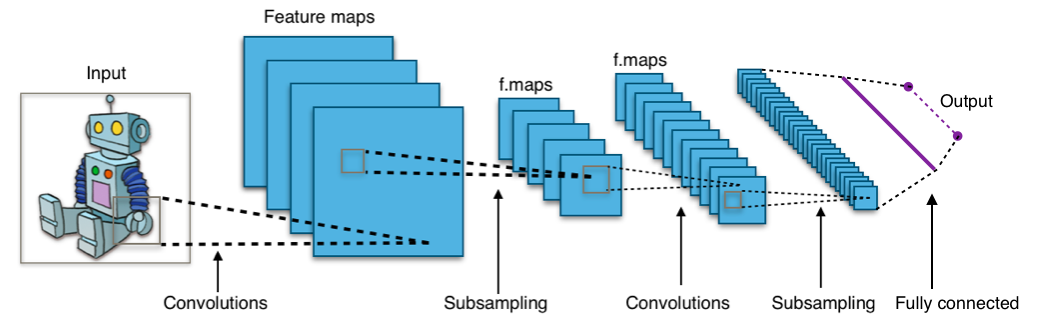
\includegraphics[scale=0.45]{images/cnn_architecture}
	\caption{An architecture of convolutional neural network}
	\label{figlncex}
\end{figure}~\\
\subsection{Convolutional layer}
Convolutional (CONV) layer computes a dot product between their weights and a small region in the input image for each small region in the input. At the output of neurons is combining the result  of the connected to local regions.\\[0.2cm]
CONV layer uses a set of learnable filters as parameters. Each filter is small spatially but extends the depth of the input. During the forward pass, the filter is slided over each pixel of the input (from left to right, top to bottom) and calculate dot product between the entries of the filter and the input at this position. During the process, we can see the response of input for each filter such as the orientation of the edge or a blotch of some color on the firt layer. With an entire set of filters in each CONV layer, we will stack these activation maps along the depth dimension and procedure the output volume.\\[0.2cm]
Instead of connecting a neurons to all neurons in the previous layer, CONV connect each neurons to only a local region of the input. The spatial extent of this connectivity is a hyperparameter called the receptive field of the neuron (equal with the number of the filter). The extent of connectivity has the depth axis is equal to the depth of the input. For example, if the input has size [32x32x3] and the filter size is [5x5] then each neuron in the CONV layer will have the weights to a [5x5x3] region in the input, and total of $5*5*3 = 75$ weights. This is the way that each neuron in CONV layer connected to the input; but how many neurons that we have in the output and how the order between the neurons. With 3 hyperparameters \textbf{depth, stride} and \textbf{zero-padding} will help us control the size of the CONV output.
\begin{itemize}
	\item \textbf{Depth}: corresponds to the number of filters we would like to use, each learning to look for something different in the input.
	\item \textbf{Stride}:  which we slide the filter. When the stride is 	1 then we move the filters one pixel at a time. If the stride is 2 (or more), then the filter will jump 2 (or more) at a time when we slide the filter.
	\item \textbf{Zero-padding}: pad the input with zeros arund the border.
\end{itemize}
We can compute the spatial size of the output through the equation:
\begin{equation}
	N = \frac{(W - F + 2P)}{S} + 1
	\label{convneuron}
\end{equation}
Where:
\begin{itemize}
	\item \textbf{W} is the input size
	\item \textbf{F} is the filter size of CONV layer neurons
	\item \textbf{P} is amount of zero padding on the border
	\item \textbf{S} is the stride.
\end{itemize}
The important of equation \ref{convneuron} is the constraint on stride. If we choose the stride inadequate, the result could be not an integer, it means that the neurons do not fit neatly and symmetrically across the input. Besides, using zero-padding also affects to the spatial size of the output. Therefore, the setting of the hyperparameters is considered to cheap, we can throw an exception or use zero pad the rest or crop the input to make it fit,etc. 
Easy to see that if a CONV layer received the input of size $[w x h x d]$, then the number of neurons is $(w * h * d)$; and if the size of the filter on each neuron is $k$, then we have $k * k * d$ weights for each neuron. And the total parameters that we need to keep on the layer is $(w * h * d) * (k * k * d)$, this number is clearly high. To reduce the number of the parameter on the layer, we can assume that if the filter is useful to compute at a position $(x_1,y_1)$, then it should be useful to compute at different postion $(x_2,y_2)$. With this way, we just need to keep unique set of weights for each depth slice(single 2-dimensional slice of depth). This technique is called parameter sharing.\\[0.2cm]
In general, the CONV layer:
\begin{itemize}
	\item Accept a input of size \textbf{$W_1$ x $H_1$ x $D_1$}
	\item Requires four hyperparameters:
		\begin{itemize}
			\item Number of filters \textbf{K}
			\item Size of filter (spatial extent) \textbf{F} (commonly F = 3)
			\item The stride \textbf{S} (commonly S = 1)
			\item The number of zero padding \textbf{P} (commonly P = 1)
		\end{itemize}
	\item The output with size of \textbf{$W_2$ x $H_2$ x $D_s$} where:
		\begin{itemize}
			\item \textbf{$W_2$ = $(W_1 - F + 2P)/S$ + $1$}
			\item \textbf{$H_2$ = $(H_1 - F + 2P)/S$ + $1$}
			\item \textbf{$D_2$ = $K$}
		\end{itemize}
	\item With parameter sharing, CONV layer store \textbf{$F * F * D_1$} weight per filter, for a total of \textbf{$(F * F * D_1) * K$} weights and \textbf{$K$} biases.
	\item In the output, the \textbf{d}-th depth slice (size \textbf{$W_2 x H_2$} is the result of performing a valid convolution on the \textbf{d}-th filter over the input volume with a stride of \textbf{$S$} and then offset by \textbf{d}-th bias.
\end{itemize}
Consider an example below (figure \ref{figconvw0}, \ref{figconvw1}), with the input is image of size \textbf{[$5$} x \textbf{$5$} x \textbf{$3$]}. The parameter of CONV layer are \textbf{K = 2, F= 3, S = 2, P = 1}, that is using two filter of size \textbf{[3x3]} and applying the stride of 2. Therefore, the size of the output volume is $(5 - 3 + 2)/2 + 1 = 3$ ([3x3x2]), and the zero padding P = 1, so making the outer border of the input with zero value. The figure \ref{figconvw0} and \ref{figconvw1} describe the process of convolution. The each the element in the output (green) is computed by elementwise multiplying the highlight input (blue) with the filter(red), summing it up, and then offsetting the sum result by the bias.
\begin{figure}[!h]
	\centering
	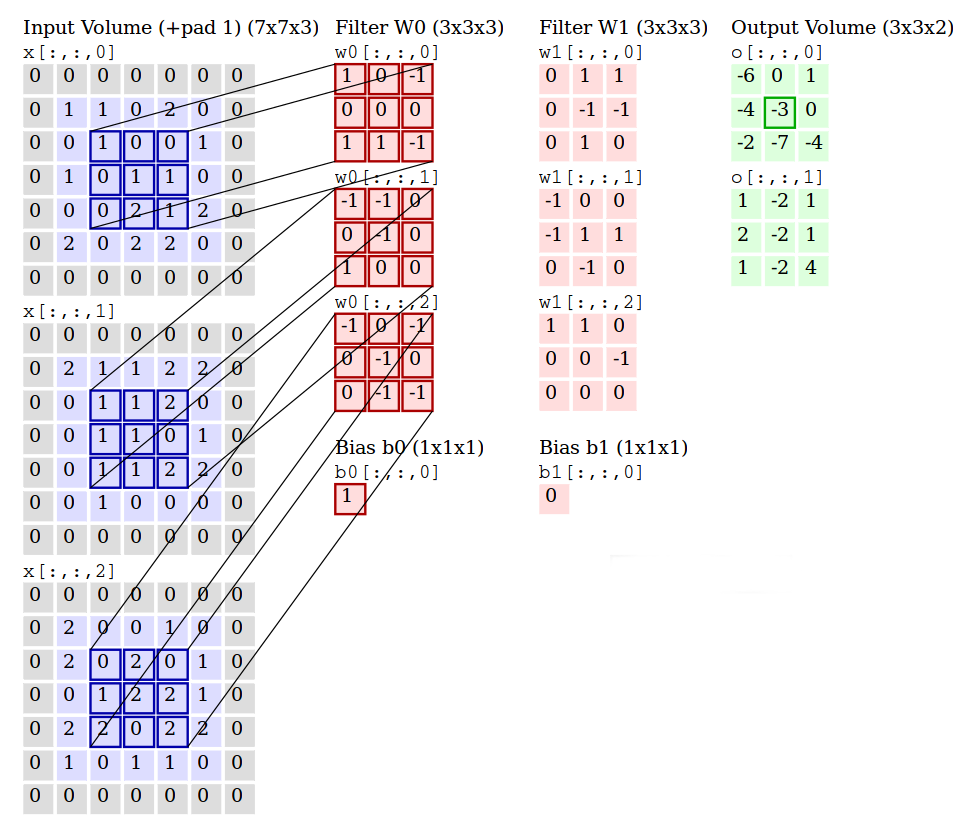
\includegraphics[scale=0.35]{images/filter_w0}
	\caption{Convolutional input with W0 filter}
	\label{figconvw0}
\end{figure}
\begin{figure}[!h]
	\centering
	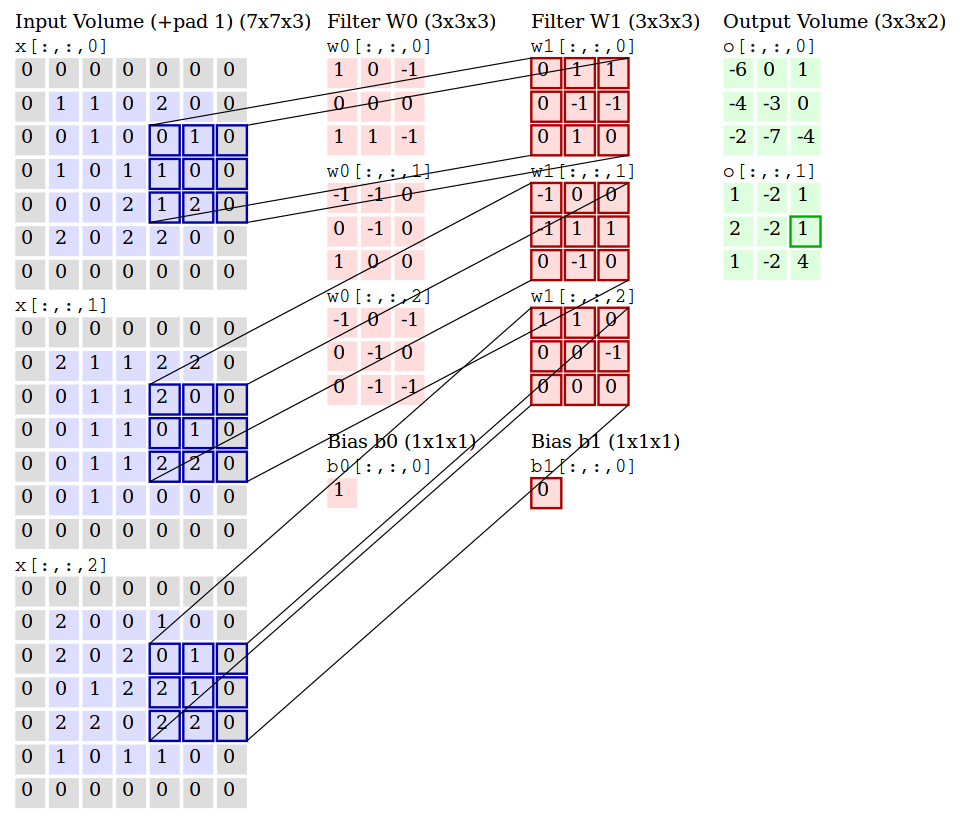
\includegraphics[scale=0.35]{images/filter_w1}
	\caption{Convolutional input with W1 filter}
	\label{figconvw1}
\end{figure}
\subsection{Pooling layer}
Pooling (POOL) layer  is another common layer in CNNs network. It is used to reduce the spatial size of the representation to reduce the quantity of the parameters and control overfitting. Hence, it performs a downsampling operation along the spatial dimensions (width, height). This operation will not affect to the depth dimension of the input. More generally, the POOL layer:
\begin{itemize}
	\item Accept a input of size \textbf{$W_1$ x $H_1$ x $D_1$}
	\item Requires two hyperparameters:
		\begin{itemize}
			\item Size of filter (spatial extent) \textbf{F} (commonly F = 4)
			\item The stride \textbf{S} (commonly S = 1)
		\end{itemize}
	\item The output with size of \textbf{$W_2$ x $H_2$ x $D_s$} where:
		\begin{itemize}
			\item \textbf{$W_2$ = $(W_1 - F)/S$ + $1$}
			\item \textbf{$H_2$ = $(H_1 - F)/S$ + $1$}
			\item \textbf{$D_2$ = $D_1$}
		\end{itemize}
	\item Note that it is not common to use zero padding for POOL layer since it computes a fixed function of the input.
\end{itemize}
The common function in POOL layer is \textbf{MAX} function and the size of filter is 2x2. The filter will slice over the input and using MAX operation over 4 number (in 2x2 region). Besides MAX function, the POOL layer can use the average function or L2-norm.
\begin{figure}[!h]
	\centering
	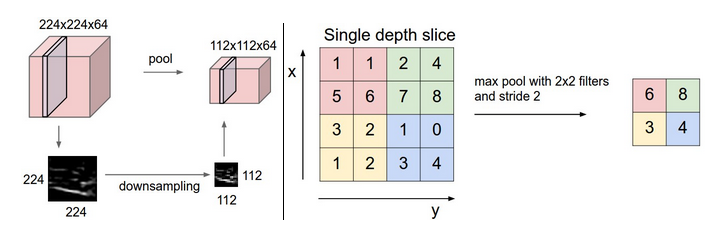
\includegraphics[scale=0.65]{images/pooling}
	\caption{A POOL layer with MAX function}
	\label{figconvw1}
\end{figure}
\subsection{Full connected layer}
Full connected (FC) layer computes the class scores of the input. The neurons in FC layer have full connections to all activations in the previous layer. Their activations can be computed with a matrix multiplication followed by a bias offset.\\[0.2cm]
The difference between CONV and FC layer is that the neurons in the CONV layer are connected only to a local region in the input and the neurons in CONV layer are sharing parameters. However, the neurons in both layers still compute the dot products (it means the functional form is identical). Therefore, it turns out that it is possible to convert between FC and CONV layer.
\begin{itemize}
	\item For any CONV layer can be become a FC layer if we implement the same forward function. The weight matrix would be a large matrix that is mostly zero except for at certain blocks where the weights in many of the blocks are equal.
	\item Conversely, a FC layer can be converted to a CONV layer by setting the filter size to be exactly the size of the input and the output will be give identical result as the initial FC layer because only a single depth column fits across the input.
\end{itemize}
\section{Case studies}
This section gives several architectures in the field of CNNs that we have.
\begin{itemize}
	\item \textbf{LeNet}: is developed by Yann Le Cun \cite{lecun1998gradient} in 1990's. It was used to read the zip code, digits.
	\item \textbf{AlexNet}: is developed by Alex Krizhevsky, Ilya Sutskever and Geoff Hinton \cite{krizhevsky2012imagenet}. This network had very similar architecture to LeNet, but was deeper, bigger and featured CONV layers stacked on top of each other.
	\item \textbf{ZF Net}: from Matthew Zeiler and Rob Fergus \cite{zeiler2014visualizing}. It was improved the AlexNet by tweaking the architecture hyperparameters (extending the size of the middle CONV layers and making the stride and the filter size on the first layer smaller).
	\item \textbf{GoogLeNet}: from Szegedy and al from Google \cite{szegedy2015going}. They develop an \textit{Inception Module} to reduce the number of parameters in the network. Additionally, they have used Average pooling instead of FC layers at the top of the CNN.
	\item \textbf{VGGNet}: is developed from Karen Simonyan and Andrew Zisserman\cite{simonyan2014very}. They show that the depth of the network is a critical component for good performance.
	\item \textbf{ResNet}: is developed by Kaiming He and al\cite{he2015deep}. The architecture of this network is missing FC layers at the end of network. It features skip connections and a heavy use of batch normalization\cite{ioffe2015batch}.
\end{itemize}
\section{Caffe framework}
Caffe is a deep learning framework that is developed by the Berkeley Vision and Learning Center (BVLC) and community contributors. Besides the supporting help user defined the network without hard-coding, easily to change the device machine (CPU or GPU), speedly, Caffe already has a large community user. These are reasons that Caffe is used in many research projects and many application in vision, speech and multimedia. This  section will describe the components and the architecture of Caffe. We also using Caffe to create a small network for classification.
\subsection{Blobs, Layers and Nets}
Deep network is a model that represented as a collection of inter-connected layers. Keep this definition, Caffe defines a network layer by layer in its model. The data through in the network called \texttt{blobs}. Blobs is the standard array and unified memory interface for the framework. The layer is the foundation of the model and computation. The net is defined as the collection of connection between the layers. The structure of blob will describe the way that information is stored and communicated in the layers and networks.
\subsubsection{Blobs}
Caffe stores and communicates data using blobs. Blobs provide a uniform memory to hold data. The blob dimensions for batches of an image are number \textbf{N} x channel \textbf{K} x height \textbf{H} x width \textbf{W}. Where:
\begin{itemize}
	\item Number N: is the batch size of the data (the number of data through the network in the same time).
	\item Channel K: is the feature dimension of image (i.e for RGB image K = 3)
	\item Width W and height H: are width and height of the image data.
\end{itemize}
In Caffe, the dimension of blob is dependent on the type and configuration of the layer.
\subsubsection{Layers}
The layer is the principle of the model and the fundamental unit of computation. Caffe has provided a lot of layer's type as convolution, pool, inner products,etc. But most of types have the same model as figure \ref{figcaffelayer}. A layer take input from the bottom connections and through the output to top connections. Each layer type defines three critical computations:
\begin{itemize}
	\item \textbf{Setup}: initialize the layer and its connections.
	\item \textbf{Forward}:  given the input from bottom connections, compute and send the output to the top connections.
	\item \textbf{Backward}: given the gradient from the top connection, compute the gradient to the input and send to the bottom connections.
\end{itemize}
\begin{figure}[!h]
	\centering
	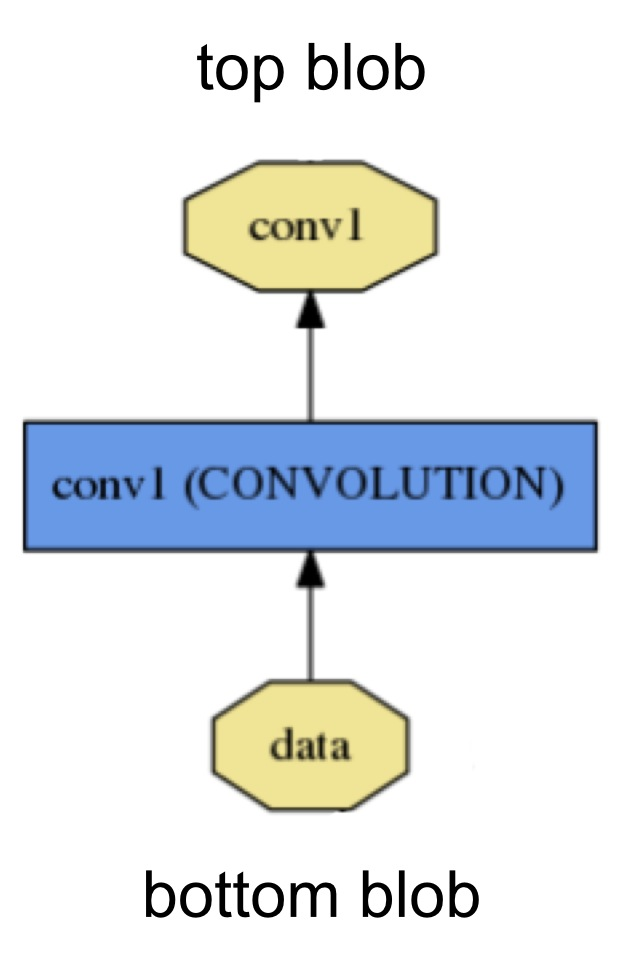
\includegraphics[scale=0.5]{images/caffelayer}
	\caption{Model of a layer in Caffe framework}
	\label{figcaffelayer}
\end{figure}
An example about declaring a layer in Caffe:\\[0.2cm]
\texttt{
layer $\lbrace \\
  \text{\tab} name: ``pool1"\\
  \text{\tab}type: ``Pooling"\\
  \text{\tab}bottom: ``conv1"\\
  \text{\tab}top: ``pool1"\\
  \text{\tab}pooling\_param \lbrace\\
  \text{\tab \tab}  pool: MAX\\
  \text{\tab \tab} kernel\_size: 2\\
  \text{\tab \tab} stride: 2\\
  \text{\tab}\rbrace\\
\rbrace$
}
\subsubsection{Nets}
The net is a set of layers connected in a computation directed acyclic graph. A net begins with a data layer that loads the data from the disk and ends with a loss layer that computes the objective of the network (such as classification, recognition,...). As simple, a net is defined as figure \ref{figcaffenet}.
\begin{figure}[!h]
	\centering
	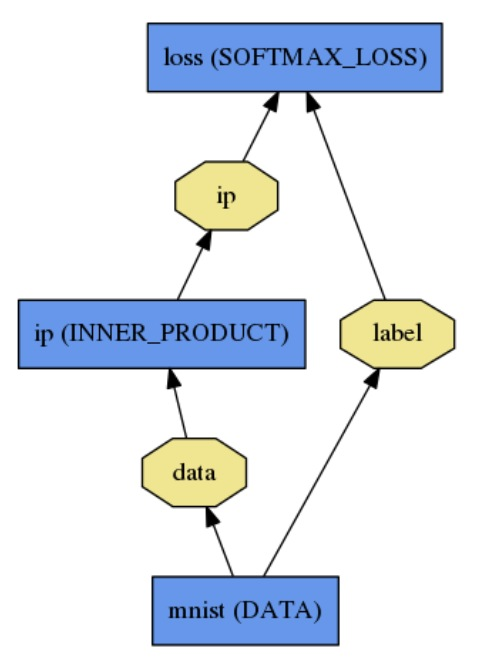
\includegraphics[scale=0.6]{images/caffenet}
	\caption{Model of a net in Caffe framework}
	\label{figcaffenet}
\end{figure}
